% Editable report converted from report/report.md. Do not replace with a PDF wrapper.
\documentclass[10pt,letterpaper]{article}
\usepackage[T1]{fontenc}
\usepackage[utf8]{inputenc}
\usepackage{lmodern}
\usepackage[margin=0.72in]{geometry}
\usepackage{microtype}
\usepackage{graphicx}
\usepackage{array,booktabs,longtable}
\usepackage{xurl}
\usepackage{needspace}
\usepackage[hidelinks]{hyperref}
\hypersetup{pdftitle={Less Formatting, Same Information},pdfauthor={Yifei Wang}}
\setlength{\parindent}{0pt}
\setlength{\parskip}{0.4em}
\setlength{\emergencystretch}{2em}
\setlength{\LTleft}{0pt}
\setlength{\LTright}{0pt}
\setlength{\LTpre}{0.4em}
\setlength{\LTpost}{0.6em}
\urlstyle{same}
\begin{document}

\begin{center}
{\LARGE\bfseries Less Formatting, Same Information}\par\medskip
Yifei Wang \textbar{} \textbf{NetID: yw251} \textbar{} Solo submission \\COMP 580 final project \textbar{} November 23, 2026 \\Code and data: \url{https://github.com/a-little-hoof/580-final}
\end{center}
\Needspace{4\baselineskip}
\section*{0. Explore and Evaluate the App}

I started by running five tasks in RUSH Lab, using a fresh NanoAgent Session for each case. The prompts were short, such as \texttt{Run the triage-log task on the edge-proxy case.} All five passed.

The installed app exposed only \texttt{deepseek/deepseek-v4-flash-0731}, abbreviated as Flash-0731 below. I could not select another model in Settings or the scored Harness interface, so I did not complete the assignment's requested comparison across different models. The \href{https://github.com/a-little-hoof/580-final/blob/main/docs/HARNESS\_CONTRACT.md}{interface audit} records this limitation.

\begingroup
\small
\setlength{\tabcolsep}{4pt}
\renewcommand{\arraystretch}{1.15}
\begin{longtable}{@{}llrrrlr@{}}
\toprule
\textbf{Task / case} & \textbf{Model} & \textbf{Cached input} & \textbf{Input tokens} & \textbf{Output tokens} & \textbf{Outcome} & \textbf{Latency (s)} \\
\midrule
\endfirsthead
\toprule
\textbf{Task / case} & \textbf{Model} & \textbf{Cached input} & \textbf{Input tokens} & \textbf{Output tokens} & \textbf{Outcome} & \textbf{Latency (s)} \\
\midrule
\endhead
\bottomrule
\endfoot
Log Triage / edge-proxy & Flash-0731 & 1,024 & 3,699 & 794 & Pass & 19.9971 \\
Cipher Crack / telegram & Flash-0731 & 6,912 & 11,581 & 1,952 & Pass & 27.4156 \\
Path Probe / quarry & Flash-0731 & 5,632 & 10,178 & 1,069 & Pass & 22.3384 \\
Regex / widget-code & Flash-0731 & 2,560 & 6,643 & 769 & Pass & 16.1301 \\
Stat Pick / sensor-drift & Flash-0731 & 2,048 & 4,793 & 1,280 & Pass & 29.1667 \\
\end{longtable}
\endgroup

Two earlier Log Triage attempts failed before reaching the task:

\begingroup
\small
\setlength{\tabcolsep}{4pt}
\renewcommand{\arraystretch}{1.15}
\begin{longtable}{@{}>{\raggedright\arraybackslash}p{.10\linewidth}>{\raggedright\arraybackslash}p{.23\linewidth}>{\raggedright\arraybackslash}p{\dimexpr.67\linewidth-4\tabcolsep\relax}@{}}
\toprule
\textbf{Attempt} & \textbf{Model} & \textbf{Result and measurements} \\
\midrule
\endfirsthead
\toprule
\textbf{Attempt} & \textbf{Model} & \textbf{Result and measurements} \\
\midrule
\endhead
\bottomrule
\endfoot
1 & Flash-0731 (configured) & OpenRouter 401: expired API key. No model response or task invocation; tokens, latency and correctness unknown. \\
2 & Flash-0731 (configured) & The same 401 error persisted after a reported key replacement. Tokens, latency and correctness unknown. \\
\end{longtable}
\endgroup

The successful token counts include both the outer chat and nested task calls, matching the app's displayed totals. Cached tokens are part of input tokens; reasoning tokens are part of output tokens. Latency measures the entire native turn. I used the recorded \texttt{valid} verdict to determine success. The \href{https://github.com/a-little-hoof/580-final/blob/main/study/task0/summaries/pilot-results.md}{pilot records} and \href{https://github.com/a-little-hoof/580-final/blob/main/docs/TRACE\_ACCOUNTING.md}{accounting notes} explain how these numbers were collected.

\Needspace{4\baselineskip}
\section*{1. Task Selection}

I selected tasks with different kinds of tool results. Log Triage identifies a fault and cites evidence from eight log lines. Cipher Crack recovers a Caesar key and plaintext. Path Probe finds a shortest route in a graph with six nodes and seven edges. Regex From Examples builds a pattern from thirteen labelled examples, then checks it against ten private examples. Stat Pick chooses and computes a statistic from eleven readings.

These cases cover text, nested records, lists and numbers. That makes them useful for testing JSON formatting: indentation takes up more space in a nested graph than in a single ciphertext string. The pilot outputs were mostly small, so I dropped the original idea of shortening large outputs and tested a simpler change: removing JSON presentation whitespace while keeping the data intact. I used the existing cases without padding them to make the savings larger.

\Needspace{4\baselineskip}
\section*{2. Task Validation}

I built a \href{https://github.com/a-little-hoof/580-final/blob/main/study/controlled/validators/validate.py}{Python validator} that checks answers without an LLM. It first checks the answer schema and confirms that the public input files have not changed. It rejects extra or missing fields, duplicate JSON keys, nonfinite numbers and booleans where numbers are required. Then it checks the answer for that task:

\begingroup
\small
\setlength{\tabcolsep}{4pt}
\renewcommand{\arraystretch}{1.15}
\begin{longtable}{@{}>{\raggedright\arraybackslash}p{.10\linewidth}>{\raggedright\arraybackslash}p{\dimexpr.90\linewidth-2\tabcolsep\relax}@{}}
\toprule
\textbf{Task} & \textbf{Correctness check} \\
\midrule
\endfirsthead
\toprule
\textbf{Task} & \textbf{Correctness check} \\
\midrule
\endhead
\bottomrule
\endfoot
Log & Require the expected fault and an accepted diagnostic line. A correct fault with an invented citation fails. Only outer evidence whitespace is ignored. \\
Cipher & Check the key and plaintext syntax, decrypt the ciphertext independently, and require agreement with the expected plaintext. Case and outer whitespace follow the upstream rules. A correct plaintext with an inconsistent key fails even if its score is 1. \\
Path & Check endpoints, edges, a simple path and its summed integer cost. Enumerate all simple paths in this six-node graph to find the optimum. Either of the two optimal routes passes. \\
Regex & Check the upstream syntax and length restrictions, then apply Python \texttt{re.fullmatch} to ten private examples in a bounded subprocess. A matching timeout is a verifier error. Passing means agreement on those examples, not proof for every possible string. \\
Stat & Require the requested statistic and compute it independently. This case uses population standard deviation, with tolerance \texttt{1e-6 * max(1, abs(expected))}. Malformed or nonrepresentable values fail. \\
\end{longtable}
\endgroup

The 23 \href{https://github.com/a-little-hoof/580-final/blob/main/study/controlled/tests/test\_validators.py}{validator tests} include valid alternatives, wrong answers, malformed JSON, huge integers, changed inputs, regex memorization and timeouts. Exhaustive path enumeration and independent arithmetic check the graph and statistics references. Log validation checks the fixed fault/citation reference. These tests cover the stated case rules; they do not guarantee correctness on new tasks.

I extracted public fixtures from pinned source literals using \texttt{ast.literal\_eval} and an explicit field allowlist. Only \texttt{input.json} and \texttt{prompt.txt} entered each evaluated workspace. Expected answers, regex holdouts and validators stayed outside the Harness VM, and internet access was disabled. The \href{https://github.com/a-little-hoof/580-final/blob/main/study/controlled/fixtures/manifest.json}{fixture manifest} records the sources and file hashes. The Python tool itself is not a sandbox; the VM provides isolation.

Coding assistance was used to develop and review the validators. The actual prompts are reproduced in the appendix and saved in \href{https://github.com/a-little-hoof/580-final/blob/main/study/controlled/validators/DEVELOPMENT.md}{DEVELOPMENT.md}.

\Needspace{4\baselineskip}
\section*{3. Your Idea and Hypothesis}

My hypothesis was that compact JSON would reduce cumulative input tokens without reducing task success. The baseline renders tool results with \texttt{json.dumps(value, ensure\_ascii=False, indent=2, allow\_nan=False)}. Compact mode replaces indentation with \texttt{separators=(',', ':')}. Both modes preserve every field, typed value, key order, array order and character inside strings.

The change should help when a result contains many nested objects or list items: removing indentation and separator spaces leaves less formatting for the model to process on later calls. It does not shorten text inside strings or remove data. I measured actual input tokens and elapsed time because a smaller JSON result does not necessarily make the whole run cheaper or faster.

\Needspace{4\baselineskip}
\section*{4. Dataset Design and Variation}

I kept one case per task and ran each condition five times. The cases give a small comparison across different data structures, rather than broad coverage of each task. Repeating a case helps show run-to-run variation, but does not add new task examples.

The CLI uses generic file tools, so two tasks needed changes in how their data was exposed. Path receives the full graph instead of discovering neighbours incrementally. Stat receives raw readings instead of a summary-only interface. Both conditions use the same adaptations, described in \href{https://github.com/a-little-hoof/580-final/blob/main/docs/ADAPTERS.md}{ADAPTERS.md}. Log, Cipher and Regex retain their source data, with only the visible Regex labels exposed. Because these interfaces differ from the native plugins, the Section 0 pilots are not the baseline for the formatting comparison.

Before running the study, I \href{https://github.com/a-little-hoof/580-final/blob/main/study/controlled/final/freeze.json}{froze} the code, package, fixtures, prompts, settings and all 50 trial requests. Seed 580 determines a shuffled order of 25 case/repetition pairs and the order of full versus compact within each pair. Each trial starts in a fresh workspace. Both modes get identical prompts and inputs, with no instruction to use a particular tool. Failed trials stay in the results and are not replaced. Provider caches cannot be reset with the workspace, so I also recorded cached tokens.

\Needspace{4\baselineskip}
\section*{5. Baseline and Fair Comparisons}

The baseline is my \href{https://github.com/a-little-hoof/580-final/tree/main/src/comp580\_agent}{Python CLI} with \texttt{--condition full}; the treatment uses the same code with \texttt{--condition compact}. I used the \href{https://github.com/RUSH-LAB/nanoagent/tree/189454718dad10404b92147b52dc07b3e6a8e598}{course NanoAgent source} to understand the app API and task contracts, then implemented the agent loop independently. Section 8 reports the full-mode baseline beside compact mode for every task.

An early full-mode installation test passed Log Triage with 2 model calls, 2,350 input tokens, 0 cached tokens, 199 output tokens and 18.06 seconds of agent time. This used an earlier package and a 4,096-token output cap, so it is excluded from the final comparison. Its \href{https://github.com/a-little-hoof/580-final/blob/main/study/controlled/development/smoke-terminal-full/capture.json}{capture} is retained with the other development tests.

All final trials used the same v0.2.0 wheel, Flash-0731 model, temperature 0, prompts, tool schemas and limits. Each attempt allowed 12 model calls and 180 seconds, with a 60-second model-request timeout and a 10-second tool timeout. The output cap was 32,768 tokens per call. Both modes applied a 64-KiB tool-result limit measured in full JSON form and a separate 2-MiB gateway-response limit. OpenRouter used the same allowed providers, DeepInfra and Nebius. The native admission ceiling was \$0.05 per attempt.

\Needspace{4\baselineskip}
\section*{6. Harness Modifications}

I installed \texttt{comp580-agent} in the RUSH Lab Harness terminal. The two commands are \texttt{rush comp580-agent --condition full} and \texttt{rush comp580-agent --condition compact}; RUSH appends the task prompt. The agent uses the supplied gateway and model with five tools: \texttt{read\_json}, \texttt{read\_file}, literal unpaginated \texttt{search\_file}, \texttt{run\_python} and \texttt{write\_answer}. It saves the final answer to \texttt{answer.json} for the verifier.

The formatting change is in \href{https://github.com/a-little-hoof/580-final/blob/main/src/comp580\_agent/tools.py}{format\_tool\_result}. The \href{https://github.com/a-little-hoof/580-final/blob/main/src/comp580\_agent/agent.py}{agent loop} applies the shared size limit before formatting, so compact mode cannot fit extra data under the limit. It saves both the raw result and the text sent to the model. \href{https://github.com/a-little-hoof/580-final/blob/main/tests/test\_compact.py}{Tests} check that both modes preserve values, Unicode and whitespace inside strings, start with identical requests, and reject the same oversized results.

Benchmark publication initially failed because RUSH Lab's answer-template builder rejected enum-only scalar schemas. I applied a small local patch that initializes these fields to \texttt{null}, matching its handling of other scalar fields. It changes no task schema, answer or verifier. Seven targeted tests and twenty existing upstream tests passed, followed by a successful native scored run. Both conditions use this patch; its \href{https://github.com/a-little-hoof/580-final/blob/main/study/controlled/development/platform-fix/README.md}{diff and runtime record} are included in the freeze.

\Needspace{4\baselineskip}
\section*{7. Evaluation Metrics}

The three primary metrics are verifier success, cumulative model input tokens and native end-to-end elapsed time. Success prevents an incomplete answer from looking efficient. Input tokens measure the expected benefit, and elapsed time measures whether that benefit makes the task faster. I also recorded cached/output tokens, tool choices, cost and agent time. Agent time starts later than native attempt time, so the table labels them separately.

For each case and condition, I report the mean and sample standard deviation over successful trials. Paired ratios use only repetitions where both modes passed and had complete measurements. Failure counts and elapsed times are reported separately, including timeouts. With five repetitions, the variation is descriptive. Caching, provider routing, network delays and the model's tool choices can still vary at temperature 0. The client makes no retries; the analysis would retain any automatic worker retries.

\Needspace{4\baselineskip}
\section*{8. Experimental Results}

The study completed all 50 trials in 50 attempts, with no worker retries or replacement trials. Full passed 23/25 and compact passed 25/25. RUSH Lab and my checker agreed on every outcome. All attempts matched the frozen package and condition. Complete usage and cost were available for 49 attempts; one timed-out request had missing usage. The \href{https://github.com/a-little-hoof/580-final/blob/main/study/controlled/final/analysis/analysis.json}{analysis}, \href{https://github.com/a-little-hoof/580-final/blob/main/study/controlled/final/analysis/trials.csv}{trial table} and \href{https://github.com/a-little-hoof/580-final/blob/main/study/controlled/final/analysis/failures.csv}{failure table} contain the full records.

Values below are \textbf{mean \textpm{} sample SD for successful trials}. Pass counts include all five trials per row; n gives the number used for the other metrics. Cached tokens are included in input tokens.

\begingroup
\small
\setlength{\tabcolsep}{4pt}
\renewcommand{\arraystretch}{1.15}
\begin{longtable}{@{}llrrrrr@{}}
\toprule
\textbf{Task / mode} & \textbf{Pass; metric n} & \textbf{Input} & \textbf{Cached subset} & \textbf{Output} & \textbf{Native s} & \textbf{Agent s} \\
\midrule
\endfirsthead
\toprule
\textbf{Task / mode} & \textbf{Pass; metric n} & \textbf{Input} & \textbf{Cached subset} & \textbf{Output} & \textbf{Native s} & \textbf{Agent s} \\
\midrule
\endhead
\bottomrule
\endfoot
Log / full & 5/5; n=5 & 2,970.0 \textpm{} 161.0 & 2,457.6 \textpm{} 229.0 & 195.8 \textpm{} 27.0 & 8.31 \textpm{} 0.79 & 5.04 \textpm{} 0.96 \\
Log / compact & 5/5; n=5 & 3,073.4 \textpm{} 188.5 & 2,355.2 \textpm{} 280.4 & 213.0 \textpm{} 22.3 & 8.60 \textpm{} 0.85 & 5.24 \textpm{} 0.83 \\
Cipher / full & 4/5; n=4 & 4,418.5 \textpm{} 16.8 & 2,816.0 \textpm{} 512.0 & 305.0 \textpm{} 28.0 & 11.44 \textpm{} 1.93 & 7.47 \textpm{} 2.34 \\
Cipher / compact & 5/5; n=5 & 4,387.6 \textpm{} 22.2 & 2,867.2 \textpm{} 457.9 & 324.6 \textpm{} 23.5 & 12.56 \textpm{} 3.45 & 8.88 \textpm{} 3.89 \\
Path / full & 5/5; n=5 & 2,619.0 \textpm{} 8.9 & 1,996.8 \textpm{} 420.7 & 231.0 \textpm{} 11.5 & 8.60 \textpm{} 1.49 & 5.54 \textpm{} 1.40 \\
Path / compact & 5/5; n=5 & 2,511.0 \textpm{} 11.0 & 1,382.4 \textpm{} 530.9 & 236.6 \textpm{} 15.7 & 9.52 \textpm{} 2.11 & 6.32 \textpm{} 1.92 \\
Regex / full & 4/5; n=4 & 3,074.5 \textpm{} 873.0 & 2,240.0 \textpm{} 1,052.9 & 545.2 \textpm{} 178.0 & 12.42 \textpm{} 3.46 & 9.35 \textpm{} 3.26 \\
Regex / compact & 5/5; n=5 & 2,825.2 \textpm{} 713.8 & 2,457.6 \textpm{} 642.6 & 537.2 \textpm{} 209.6 & 13.54 \textpm{} 1.98 & 10.33 \textpm{} 1.76 \\
Stat / full & 5/5; n=5 & 4,519.8 \textpm{} 361.0 & 2,969.6 \textpm{} 642.6 & 645.6 \textpm{} 65.1 & 13.39 \textpm{} 2.29 & 10.03 \textpm{} 2.27 \\
Stat / compact & 5/5; n=5 & 4,207.0 \textpm{} 332.9 & 3,020.8 \textpm{} 662.6 & 625.0 \textpm{} 92.9 & 17.37 \textpm{} 4.68 & 14.08 \textpm{} 4.74 \\
\end{longtable}
\endgroup

The two failures were both in full mode. Cipher repetition 2 returned the correct plaintext with an inconsistent key, so it failed despite a score of 1.0. It used 4,433 input tokens and took 10.42 seconds. Regex repetition 3 timed out on its third model request and left an unfilled answer template. The attempt took 107.39 seconds. Its first two calls used 2,638 input, 2,304 cached and 3,827 output tokens; complete totals are unknown. Including these failures, Cipher's full/compact mean times were 11.23/12.56 seconds, and Regex's were 31.42/13.54 seconds. The large Regex difference comes mainly from that one timeout.

\begin{center}\begin{minipage}{\linewidth}
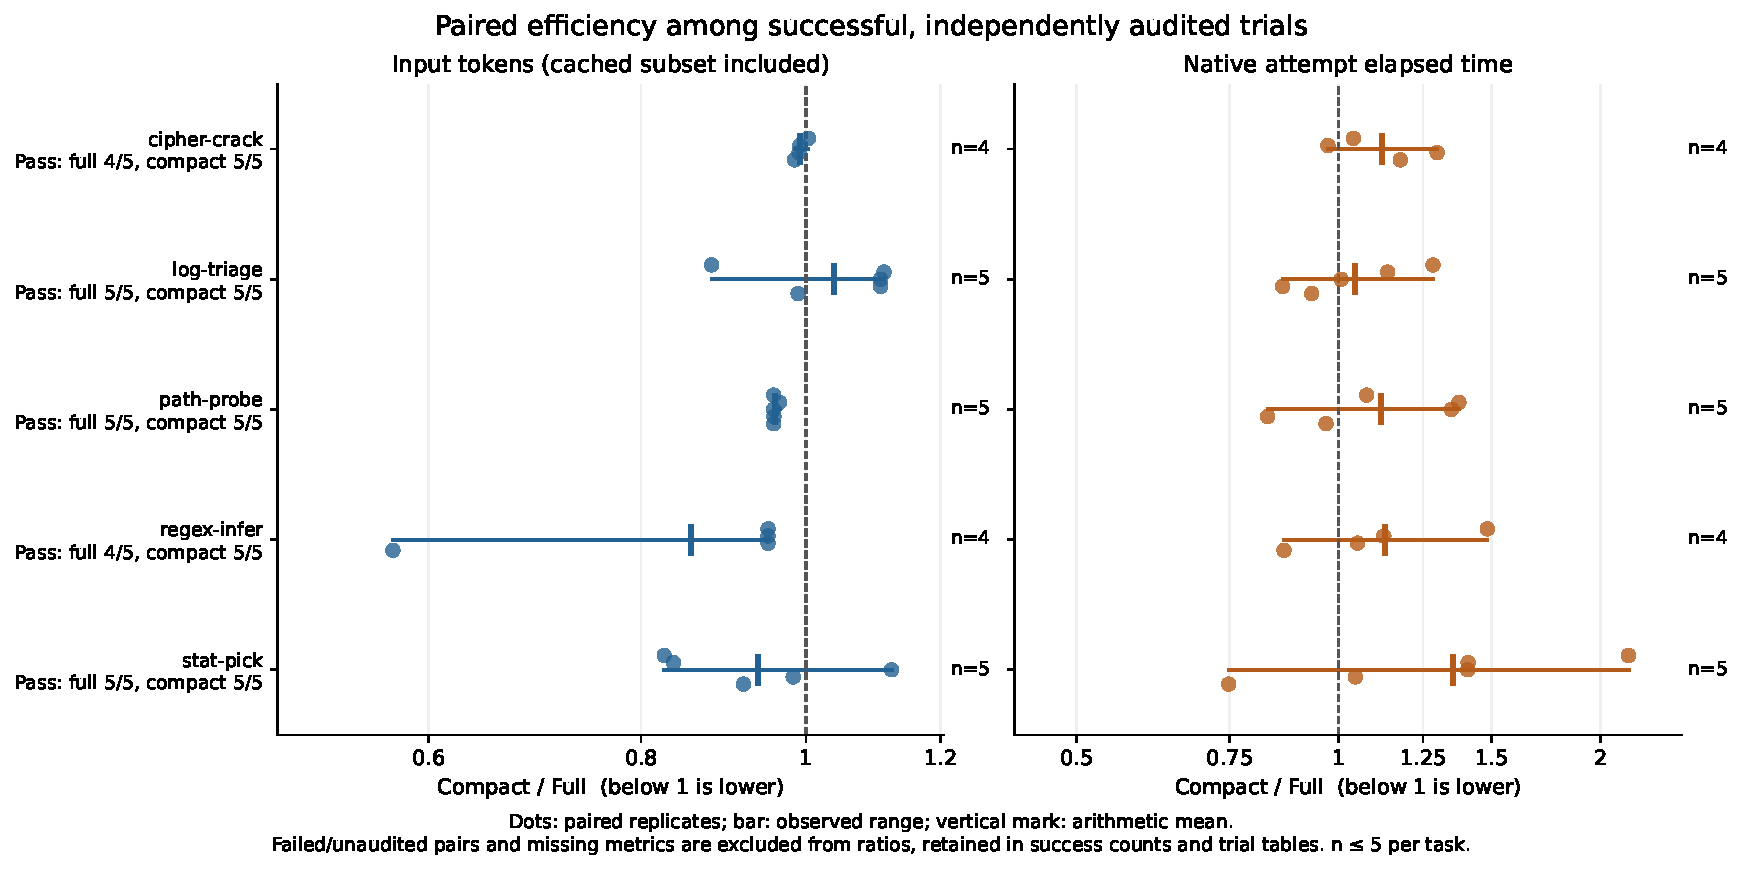
\includegraphics[width=\linewidth]{main-comparison.pdf}
\par\smallskip{\small \textbf{Figure 1.} Each dot is a compact/full ratio for one successful pair. The mark shows the mean and the line shows the observed range. Cipher and Regex have four pairs; the others have five. These are means of paired ratios, not ratios of the table means. A ratio below 1 favours compact mode.}
\end{minipage}\end{center}

\textbf{Log Triage.} Both modes passed all five runs, but compact used 103.4 more input tokens on average. Each ordinary structured log result shrank from 788 to 703 bytes. However, compact made three extra \texttt{read\_file} calls across its trials, compared with one in full mode. Those choices happened before the first formatted result, so formatting could not have caused the imbalance. Both modes used two model calls per run. Extra file reads outweighed the small formatting savings. Compact was also slightly slower on average.

\textbf{Cipher Crack.} Full passed four runs and compact passed five. All runs used three model calls and the same tools: \texttt{read\_json}, \texttt{run\_python} and \texttt{write\_answer}. Compact removed only 37 delivered bytes per run because most of the content was inside strings. Across the four successful pairs, it saved an average of 33 input tokens. For this task, the formatting change made little difference to token usage and did not improve average speed.

\textbf{Path Probe.} Both modes passed every run with the same two-call sequence: read the graph, then write the route. The graph result shrank from 660 to 311 bytes, or 52.9\%. Total input tokens fell by 108 on average, about 4.1\%. This was the clearest result because the tool sequence stayed the same and the token reduction was consistent. The saving in total input was much smaller than the saving in graph bytes because prompts and tool schemas also take up context. Native time rose from 8.60 to 9.52 seconds on average. Compact also had fewer cached tokens, and mean reported cost rose from \$0.000175 to \$0.000221.

\textbf{Regex From Examples.} Full passed four runs and compact passed five. Three successful pairs used two model calls in both modes and saved exactly 132 input tokens, about 5\%. In the fourth pair, full made an extra Python/model round, and compact saved 1,878 tokens. That one difference pulled the mean paired saving up to 14.5\%. The structured example result itself shrank from 981 to 510 bytes. Compact was still slower on average across the four successful pairs. The pair containing the full-mode timeout is excluded from token ratios, but both outcomes remain in the pass counts.

\textbf{Stat Pick.} Both modes passed every run with three model calls. Compact used 312.8 fewer input tokens on average, but tool choices varied. Full made three extra \texttt{read\_file} calls and one \texttt{search\_file} call, while compact made one extra \texttt{read\_file} call. As with Log, these choices preceded the first formatted result. Some of the observed saving therefore comes from different reads rather than JSON whitespace. Mean native time increased from 13.39 to 17.37 seconds. This task did not show a dependable speed benefit.

\Needspace{4\baselineskip}
\section*{9. Conclusion}

Compact JSON saved some input tokens, but it did not make these tasks consistently faster. Path showed the clearest benefit: about 4.1\% fewer input tokens with the same tool sequence. Regex showed about 5\% savings when both modes used two calls. Cipher changed little, while extra reads complicated the Log and Stat results. Compact passed 25/25 compared with full's 23/25, but two failures in this small study are not enough to claim better reliability. My conclusion is limited to these five cases and one model: compact formatting is a small token-saving change for structured results, with no demonstrated general speedup.

\Needspace{4\baselineskip}
\section*{Appendix: Reproduction and validator prompts}

The CLI requires Python 3.12 or newer and uses only the standard library at runtime. The \href{https://github.com/a-little-hoof/580-final/blob/main/docs/REPRODUCE.md}{reproduction guide} explains how to install it, run the offline tests, regenerate the analysis and build this report through the \href{https://github.com/a-little-hoof/580-final/blob/main/Makefile}{Makefile}. The repository contains the frozen wheel, code and input hashes, run order, raw evidence and plotting script. There are 121 offline tests; without the optional upstream checkouts, one fixture-rebuild test is skipped. The source ZIP provides the assignment's fallback code package.

The following are the actual prompts used to implement and review the validators. They are preserved verbatim, including their shorthand wording. The \href{https://github.com/a-little-hoof/580-final/blob/main/study/controlled/development/prompts.jsonl}{prompt record} also includes the user's choice of compact formatting.

\begin{quote}\small
User approved lossless compact formatting. Implement public fixtures + private deterministic validators and meaningful tests, exclusively under study/controlled/\{fixtures,validators,tests\} and docs/ADAPTERS.md. Read draft and contracts. Use AST literal extraction explicit allowlist; no plugin execution or model calls. Each case directory input.json plus prompt.txt with public task definitions/schema/case exact data. Same tasks/cases as pilots; clearly fullgraph/rawstats adaptation. Keep private validator reference data outside publicfixtures/package. Validate typed answer and integrity, reproduce upstream acceptance nuances. Need manifest input hashes/source versions/extraction provenance/license. Do not edit projectroot plan/README. Communicate interface/files for baselineagent. Do not include known answer/hiddenlabels in prompts or fixture files.
\end{quote}

\begin{quote}\small
Interface approved. Coordinate manifest shape with inspect\_path\_stat\_regex agent implementing dryrun benchmarkhelper. Fixtureprompt identical conditions; original Session caseprompt difference declared. Need do not force full outputs or use read\_json specifically; natural prompt says input file. Ensure license source notices and private truthisolated.
\end{quote}

\begin{quote}\small
Early validatorreview looks good. Please test huge integer stat.value (e.g10**1000) causing OverflowError subtractfloat; should deterministicreject false notuncaughtcrash. Sourceinterface metadata/hashesgood. Root wrote study/controlled/prepare\_workspace.py twofileallowlist newdironly, noconflict. Final testsinclude missing/modifiedpromptinput, extra fields andtypeboolcost, syntacticinvalidduplicate/NaN/overflowJSON.
\end{quote}

\end{document}
